\documentclass{article}
\usepackage{graphicx}
\usepackage[export]{adjustbox}
\usepackage{tabularx}  %better tables
\usepackage[margin=1in]{geometry}
\usepackage{hyperref}
\usepackage{tikz}
\usepackage{multicol}

\title{Homework 5 CSCI 451}
\author{Nicholas Rust}
\date{due: 03 December 2019}

\begin{document}
\maketitle

\section{Exercise 7.6.1 (pg 193)}

\begin{multicols}{2}
\tikzset{every picture/.style={line width=0.75pt}} %set default line width to 0.75pt        

\begin{tikzpicture}[x=0.75pt,y=0.75pt,yscale=-1,xscale=1]
%uncomment if require: \path (0,300); %set diagram left start at 0, and has height of 300

%Shape: Rectangle [id:dp34620925499172717] 
\draw   (202,50) -- (247,50) -- (247,90) -- (202,90) -- cycle ;
%Shape: Rectangle [id:dp952632327601173] 
\draw   (428,50) -- (473,50) -- (473,90) -- (428,90) -- cycle ;
%Shape: Rectangle [id:dp8934132786852836] 
\draw   (313,172) -- (358,172) -- (358,212) -- (313,212) -- cycle ;
%Straight Lines [id:da7200763263461912] 
\draw    (226,90) -- (313,191) ;


%Straight Lines [id:da9365103585365722] 
\draw    (247,69) -- (428,70) ;


%Straight Lines [id:da04815292916630265] 
\draw    (454,89) -- (358,193) ;



% Text Node
\draw (224.5,70) node   {$S_{1}$};
% Text Node
\draw (450.5,70) node   {$S_{3}$};
% Text Node
\draw (335.5,192) node   {$S_{2}$};
% Text Node
\draw (253,152) node  [align=left] {2};
% Text Node
\draw (339,49) node  [align=left] {3};
% Text Node
\draw (424,154) node  [align=left] {3};

\end{tikzpicture}

\tikzset{every picture/.style={line width=0.75pt}} %set default line width to 0.75pt        

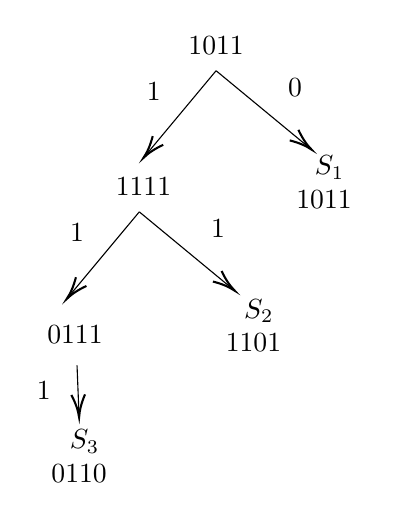
\begin{tikzpicture}[x=0.75pt,y=0.75pt,yscale=-1,xscale=1]
%uncomment if require: \path (0,300); %set diagram left start at 0, and has height of 300

%Straight Lines [id:da4159343546133505] 
\draw    (163,54) -- (207.46,90.73) ;
\draw [shift={(209,92)}, rotate = 219.56] [color={rgb, 255:red, 0; green, 0; blue, 0 }  ][line width=0.75]    (10.93,-3.29) .. controls (6.95,-1.4) and (3.31,-0.3) .. (0,0) .. controls (3.31,0.3) and (6.95,1.4) .. (10.93,3.29)   ;

%Straight Lines [id:da6872341646291027] 
\draw    (163,54) -- (129.28,94.46) ;
\draw [shift={(128,96)}, rotate = 309.81] [color={rgb, 255:red, 0; green, 0; blue, 0 }  ][line width=0.75]    (10.93,-3.29) .. controls (6.95,-1.4) and (3.31,-0.3) .. (0,0) .. controls (3.31,0.3) and (6.95,1.4) .. (10.93,3.29)   ;

%Straight Lines [id:da9919664184660275] 
\draw    (126,122) -- (170.46,158.73) ;
\draw [shift={(172,160)}, rotate = 219.56] [color={rgb, 255:red, 0; green, 0; blue, 0 }  ][line width=0.75]    (10.93,-3.29) .. controls (6.95,-1.4) and (3.31,-0.3) .. (0,0) .. controls (3.31,0.3) and (6.95,1.4) .. (10.93,3.29)   ;

%Straight Lines [id:da7065242689125987] 
\draw    (126,122) -- (92.28,162.46) ;
\draw [shift={(91,164)}, rotate = 309.81] [color={rgb, 255:red, 0; green, 0; blue, 0 }  ][line width=0.75]    (10.93,-3.29) .. controls (6.95,-1.4) and (3.31,-0.3) .. (0,0) .. controls (3.31,0.3) and (6.95,1.4) .. (10.93,3.29)   ;

%Straight Lines [id:da031050249931263263] 
\draw    (96,196) -- (96.92,219) ;
\draw [shift={(97,221)}, rotate = 267.71] [color={rgb, 255:red, 0; green, 0; blue, 0 }  ][line width=0.75]    (10.93,-3.29) .. controls (6.95,-1.4) and (3.31,-0.3) .. (0,0) .. controls (3.31,0.3) and (6.95,1.4) .. (10.93,3.29)   ;


% Text Node
\draw (215,109) node   {$ \begin{array}{l}
\ \ S_{1}\\
1011
\end{array}$};
% Text Node
\draw (163,42) node   {$1011$};
% Text Node
\draw (181,178) node   {$ \begin{array}{l}
\ \ S_{2}\\
1101
\end{array}$};
% Text Node
\draw (133,64) node  [align=left] {1};
% Text Node
\draw (201,62) node  [align=left] {0};
% Text Node
\draw (128,110) node   {$1111$};
% Text Node
\draw (96,132) node  [align=left] {1};
% Text Node
\draw (164,130) node  [align=left] {1};
% Text Node
\draw (95,181) node   {$0111$};
% Text Node
\draw (80,208) node  [align=left] {1};
% Text Node
\draw (97,241) node   {$ \begin{array}{l}
\ \ S_{3}\\
0110
\end{array}$};


\end{tikzpicture}

\end{multicols}

This does appear to be one of the maximum parsimony trees as $S_3$ is an equal number of changes from both $S_1$ and $S_2$.

\begin{multicols}{2}
\section{Exercise 7.6.3 (pg 193)}

\tikzset{every picture/.style={line width=0.75pt}} %set default line width to 0.75pt        

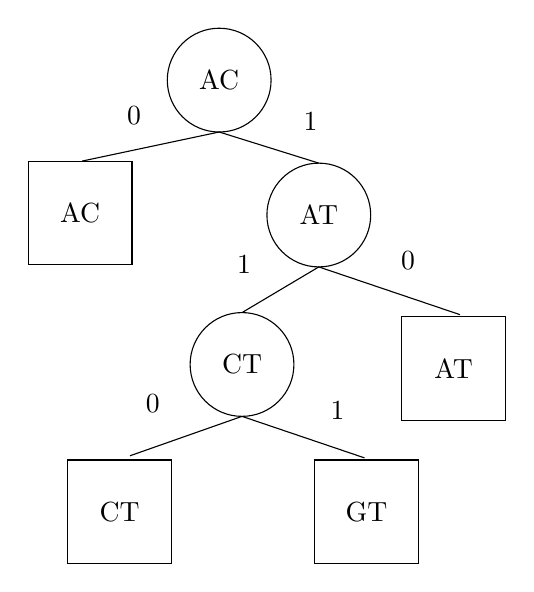
\begin{tikzpicture}[x=0.75pt,y=0.75pt,yscale=-1,xscale=1]
%uncomment if require: \path (0,300); %set diagram left start at 0, and has height of 300

%Shape: Circle [id:dp8032871031265186] 
\draw   (289,41) .. controls (289,27.19) and (300.19,16) .. (314,16) .. controls (327.81,16) and (339,27.19) .. (339,41) .. controls (339,54.81) and (327.81,66) .. (314,66) .. controls (300.19,66) and (289,54.81) .. (289,41) -- cycle ;
%Shape: Circle [id:dp6881005088428123] 
\draw   (337,106) .. controls (337,92.19) and (348.19,81) .. (362,81) .. controls (375.81,81) and (387,92.19) .. (387,106) .. controls (387,119.81) and (375.81,131) .. (362,131) .. controls (348.19,131) and (337,119.81) .. (337,106) -- cycle ;
%Shape: Circle [id:dp752896447996085] 
\draw   (300,178) .. controls (300,164.19) and (311.19,153) .. (325,153) .. controls (338.81,153) and (350,164.19) .. (350,178) .. controls (350,191.81) and (338.81,203) .. (325,203) .. controls (311.19,203) and (300,191.81) .. (300,178) -- cycle ;
%Shape: Square [id:dp5375556645017805] 
\draw   (222,80) -- (272,80) -- (272,130) -- (222,130) -- cycle ;
%Shape: Square [id:dp058317332363127306] 
\draw   (402,155) -- (452,155) -- (452,205) -- (402,205) -- cycle ;
%Shape: Square [id:dp03704790191058516] 
\draw   (241,224) -- (291,224) -- (291,274) -- (241,274) -- cycle ;
%Shape: Square [id:dp005257366096731775] 
\draw   (360,224) -- (410,224) -- (410,274) -- (360,274) -- cycle ;
%Straight Lines [id:da10826640726638193] 
\draw    (314,66) -- (248,80) ;


%Straight Lines [id:da9140159521777942] 
\draw    (362,81) -- (314,66) ;


%Straight Lines [id:da526530785747245] 
\draw    (362,131) -- (325,153) ;


%Straight Lines [id:da7557468354357798] 
\draw    (362,131) -- (430,154) ;


%Straight Lines [id:da5700559399551837] 
\draw    (325,203) -- (384,223) ;


%Straight Lines [id:da9869240644433085] 
\draw    (325,203) -- (271,222) ;



% Text Node
\draw (314,41) node  [align=left] {AC};
% Text Node
\draw (247,105) node  [align=left] {AC};
% Text Node
\draw (362,106) node  [align=left] {AT};
% Text Node
\draw (427,180) node  [align=left] {AT};
% Text Node
\draw (325,178) node  [align=left] {CT};
% Text Node
\draw (266,249) node  [align=left] {CT};
% Text Node
\draw (385,249) node  [align=left] {GT};
% Text Node
\draw (273,58) node  [align=left] {0};
% Text Node
\draw (358,61) node  [align=left] {1};
% Text Node
\draw (326,130) node  [align=left] {1};
% Text Node
\draw (371,200) node  [align=left] {1};
% Text Node
\draw (282,197) node  [align=left] {0};
% Text Node
\draw (405,128) node  [align=left] {0};

\end{tikzpicture}

The parsimony length appears to be 3.

\section{Exercise 7.6.4 (pg 194)}
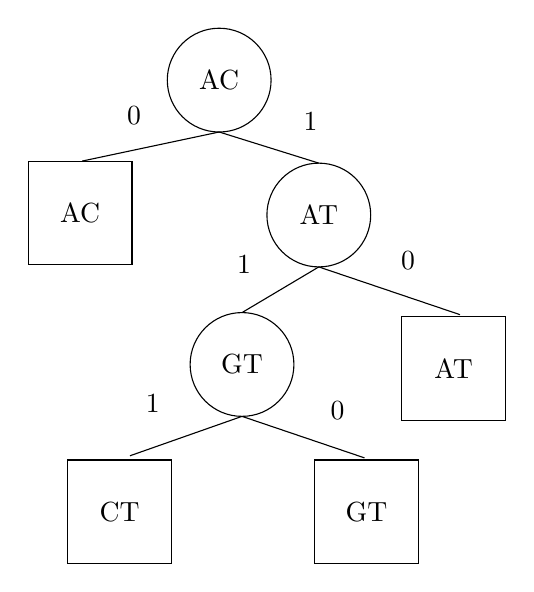
\begin{tikzpicture}[x=0.75pt,y=0.75pt,yscale=-1,xscale=1]
%uncomment if require: \path (0,300); %set diagram left start at 0, and has height of 300

%Shape: Circle [id:dp8032871031265186] 
\draw   (289,41) .. controls (289,27.19) and (300.19,16) .. (314,16) .. controls (327.81,16) and (339,27.19) .. (339,41) .. controls (339,54.81) and (327.81,66) .. (314,66) .. controls (300.19,66) and (289,54.81) .. (289,41) -- cycle ;
%Shape: Circle [id:dp6881005088428123] 
\draw   (337,106) .. controls (337,92.19) and (348.19,81) .. (362,81) .. controls (375.81,81) and (387,92.19) .. (387,106) .. controls (387,119.81) and (375.81,131) .. (362,131) .. controls (348.19,131) and (337,119.81) .. (337,106) -- cycle ;
%Shape: Circle [id:dp752896447996085] 
\draw   (300,178) .. controls (300,164.19) and (311.19,153) .. (325,153) .. controls (338.81,153) and (350,164.19) .. (350,178) .. controls (350,191.81) and (338.81,203) .. (325,203) .. controls (311.19,203) and (300,191.81) .. (300,178) -- cycle ;
%Shape: Square [id:dp5375556645017805] 
\draw   (222,80) -- (272,80) -- (272,130) -- (222,130) -- cycle ;
%Shape: Square [id:dp058317332363127306] 
\draw   (402,155) -- (452,155) -- (452,205) -- (402,205) -- cycle ;
%Shape: Square [id:dp03704790191058516] 
\draw   (241,224) -- (291,224) -- (291,274) -- (241,274) -- cycle ;
%Shape: Square [id:dp005257366096731775] 
\draw   (360,224) -- (410,224) -- (410,274) -- (360,274) -- cycle ;
%Straight Lines [id:da10826640726638193] 
\draw    (314,66) -- (248,80) ;


%Straight Lines [id:da9140159521777942] 
\draw    (362,81) -- (314,66) ;


%Straight Lines [id:da526530785747245] 
\draw    (362,131) -- (325,153) ;


%Straight Lines [id:da7557468354357798] 
\draw    (362,131) -- (430,154) ;


%Straight Lines [id:da5700559399551837] 
\draw    (325,203) -- (384,223) ;


%Straight Lines [id:da9869240644433085] 
\draw    (325,203) -- (271,222) ;



% Text Node
\draw (314,41) node  [align=left] {AC};
% Text Node
\draw (247,105) node  [align=left] {AC};
% Text Node
\draw (362,106) node  [align=left] {AT};
% Text Node
\draw (427,180) node  [align=left] {AT};
% Text Node
\draw (325,178) node  [align=left] {GT};
% Text Node
\draw (266,249) node  [align=left] {CT};
% Text Node
\draw (385,249) node  [align=left] {GT};
% Text Node
\draw (273,58) node  [align=left] {0};
% Text Node
\draw (358,61) node  [align=left] {1};
% Text Node
\draw (326,130) node  [align=left] {1}; % 1
% Text Node
\draw (371,200) node  [align=left] {0}; % 1
% Text Node
\draw (282,197) node  [align=left] {1};
% Text Node
\draw (405,128) node  [align=left] {0}; % 0

\end{tikzpicture}

Note the CT internal node is now GT, PL = 3.

\end{multicols}
\section{Exercise 4.8.1 (pg 105)}




\tikzset{every picture/.style={line width=0.75pt}} %set default line width to 0.75pt        

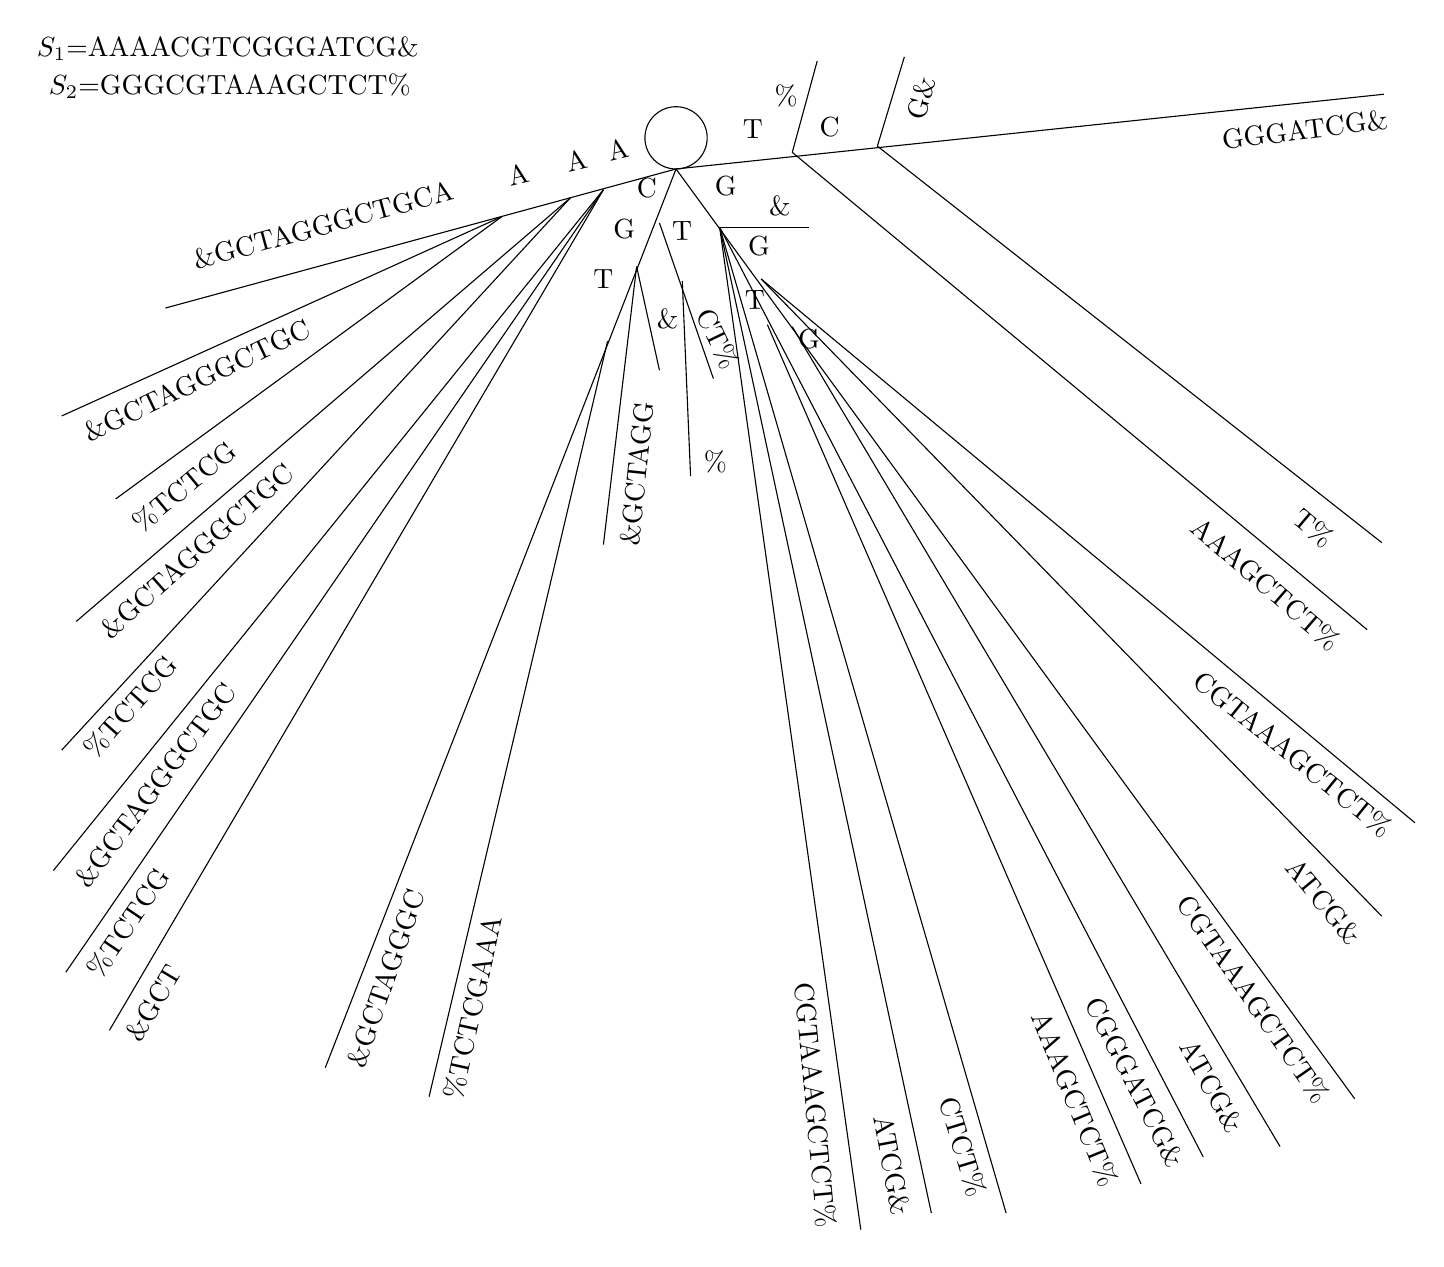
\begin{tikzpicture}[x=0.75pt,y=0.75pt,yscale=-1,xscale=1]
%uncomment if require: \path (0,979); %set diagram left start at 0, and has height of 979

%Straight Lines [id:da4609083131857874] 
\draw    (311,328) -- (65,395) ;


%Shape: Circle [id:dp01067243217799374] 
\draw   (296,313) .. controls (296,304.72) and (302.72,298) .. (311,298) .. controls (319.28,298) and (326,304.72) .. (326,313) .. controls (326,321.28) and (319.28,328) .. (311,328) .. controls (302.72,328) and (296,321.28) .. (296,313) -- cycle ;
%Straight Lines [id:da8898503038870013] 
\draw    (227,351) -- (15,447) ;


%Straight Lines [id:da8422111645527942] 
\draw    (260,342) -- (22,546) ;


%Straight Lines [id:da7066761829942521] 
\draw    (276,338) -- (11,666) ;


%Straight Lines [id:da5993216460146737] 
\draw    (227,351) -- (41,487) ;


%Straight Lines [id:da5375682294285766] 
\draw    (260,342) -- (15,608) ;


%Straight Lines [id:da8010807768264783] 
\draw    (276,338) -- (17,715) ;


%Straight Lines [id:da35407722082002] 
\draw    (276,338) -- (38,743) ;


%Straight Lines [id:da39684449479898887] 
\draw    (311,328) -- (142,761) ;


%Straight Lines [id:da7922639837528037] 
\draw    (303,354) -- (329,429) ;


%Straight Lines [id:da0576711774202574] 
\draw    (314,382) -- (318,476) ;


%Straight Lines [id:da9862399283112722] 
\draw    (292,375) -- (303,425) ;


%Straight Lines [id:da37460439034158544] 
\draw    (292,375) -- (276,509) ;


%Straight Lines [id:da8675327460343757] 
\draw    (278,411) -- (192,775) ;


%Straight Lines [id:da34579383195923097] 
\draw    (311,328) -- (638,776) ;


%Straight Lines [id:da8741950094128902] 
\draw    (367,404) -- (602,799) ;


%Straight Lines [id:da5149859191571581] 
\draw    (332,356) -- (375,356) ;


%Straight Lines [id:da3779551620195052] 
\draw    (332,356) -- (565,804) ;


%Straight Lines [id:da16403127296384223] 
\draw    (355,403) -- (535,817) ;


%Straight Lines [id:da9952532147457251] 
\draw    (332,356) -- (470,831) ;


%Straight Lines [id:da2980620074148511] 
\draw    (352,381) -- (651,688) ;


%Straight Lines [id:da9582111874863677] 
\draw    (332,356) -- (434,831) ;


%Straight Lines [id:da366825279242708] 
\draw    (352,381) -- (667,643) ;


%Straight Lines [id:da1852878580491497] 
\draw    (332,356) -- (400,839) ;


%Straight Lines [id:da3967473564433581] 
\draw    (311,328) -- (652,292) ;


%Straight Lines [id:da806349911800657] 
\draw    (367,320) -- (379,276) ;


%Straight Lines [id:da7072527405599934] 
\draw    (408,317) -- (651,508) ;


%Straight Lines [id:da23080746053522738] 
\draw    (367,320) -- (644,550) ;


%Straight Lines [id:da8287091498119886] 
\draw    (408,317) -- (421,274) ;



% Text Node
\draw (141,355) node [rotate=-344.74] [align=left] {$ $\&GCTAGGGCTGCA};
% Text Node
\draw (80,430) node [rotate=-334.41] [align=left] {\&GCTAGGGCTGC};
% Text Node
\draw (235,331) node [rotate=-346.47] [align=left] {A};
% Text Node
\draw (263,324) node [rotate=-346.47] [align=left] {A};
% Text Node
\draw (283,319) node [rotate=-346.47] [align=left] {A};
% Text Node
\draw (80,512) node [rotate=-318.46] [align=left] {\&GCTAGGGCTGC};
% Text Node
\draw (60,625) node [rotate=-307.16] [align=left] {\&GCTAGGGCTGC};
% Text Node
\draw (59,730) node [rotate=-300.85] [align=left] {\&GCT};
% Text Node
\draw (74,481) node [rotate=-320.54] [align=left] {\%TCTCG};
% Text Node
\draw (48,587) node [rotate=-311.71] [align=left] {\%TCTCG};
% Text Node
\draw (47,691) node [rotate=-303.96] [align=left] {\%TCTCG};
% Text Node
\draw (297,337) node  [align=left] {C};
% Text Node
\draw (286,357) node  [align=left] {G};
% Text Node
\draw (314,358) node [rotate=-359] [align=left] {T};
% Text Node
\draw (95,270) node  [align=left] {$\displaystyle S_{1}$=AAAACGTCGGGATCG\&};
% Text Node
\draw (96,288) node  [align=left] {$\displaystyle S_{2}$=GGGCGTAAAGCTCT\%};
% Text Node
\draw (331,410) node [rotate=-64.29] [align=left] {CT\%};
% Text Node
\draw (330,469) node  [align=left] {\%};
% Text Node
\draw (307,400) node  [align=left] {\&};
% Text Node
\draw (276,381) node  [align=left] {T};
% Text Node
\draw (171,718) node [rotate=-289.26] [align=left] {\&GCTAGGGC};
% Text Node
\draw (213,732) node [rotate=-282.49] [align=left] {\%TCTCGAAA};
% Text Node
\draw (292,475) node [rotate=-276.03] [align=left] {\&GCTAGG};
% Text Node
\draw (335,336) node  [align=left] {G};
% Text Node
\draw (351,365) node  [align=left] {G};
% Text Node
\draw (375,410) node  [align=left] {G};
% Text Node
\draw (589,728) node [rotate=-55.26] [align=left] {CGTAAAGCTCT\%};
% Text Node
\draw (569,770) node [rotate=-60.77] [align=left] {ATCG\&};
% Text Node
\draw (361,346) node  [align=left] {\&};
% Text Node
\draw (349,391) node [rotate=-359] [align=left] {T};
% Text Node
\draw (532,768) node [rotate=-63.05] [align=left] {CGGGATCG\&};
% Text Node
\draw (503,776) node [rotate=-67.69] [align=left] {AAAGCTCT\%};
% Text Node
\draw (449,799) node [rotate=-73.13] [align=left] {CTCT\%};
% Text Node
\draw (623,681) node [rotate=-50.4] [align=left] {ATCG\&};
% Text Node
\draw (415,808) node [rotate=-79.4] [align=left] {ATCG\&};
% Text Node
\draw (608,610) node [rotate=-38.9] [align=left] {CGTAAAGCTCT\%};
% Text Node
\draw (378,779) node [rotate=-84.72] [align=left] {CGTAAAGCTCT\%};
% Text Node
\draw (348,309) node  [align=left] {T};
% Text Node
\draw (385,308) node  [align=left] {C};
% Text Node
\draw (364,293) node  [align=left] {\%};
% Text Node
\draw (618,501) node [rotate=-40.29] [align=left] {T\%};
% Text Node
\draw (614,309) node [rotate=-352.65] [align=left] {GGGATCG\&};
% Text Node
\draw (595,528) node [rotate=-40.81] [align=left] {AAAGCTCT\%};
% Text Node
\draw (429,294) node [rotate=-285.35] [align=left] {G\&};

\end{tikzpicture}

MUMs: {CGT, GGG, AAA}.

Sorry this is a bit of a mess, but AAA is directly off the left-hand side, and GGG is in the large mess under the T branch, CGT is directly to the left of the G branch. Each of these series of letters has exactly two children, one from each string and is the LCA.
\section{Exercise 4.8.2 (pg 105)}
MUMs: {CGT, GGG}

\begin{figure}
	\section{Sample Output}
    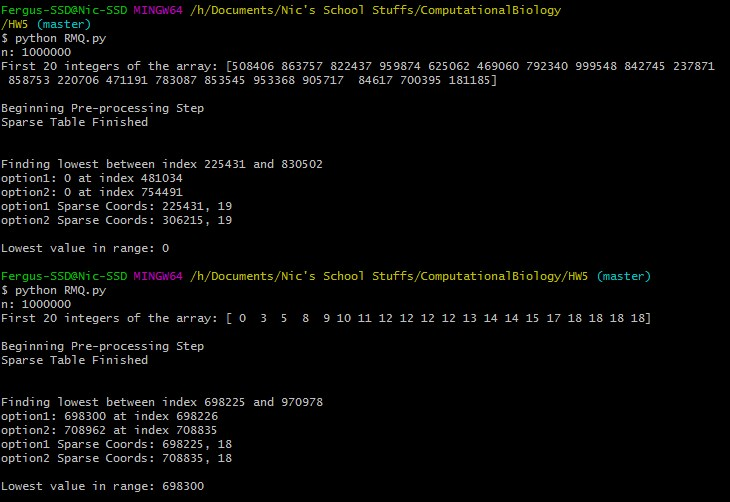
\includegraphics[width=\textwidth,center]{HW5_SampleOutput.jpg}
    \caption{Program Output}
\end{figure}


\end{document}